
\section{Einleitung}
Durch das Anschließen des Geiger-Müller-Zählrohrs an einen elektronischen Impulszähler
kann die Intensität ionisierender Strahlungen gemessen werden. Wird im Inneren des Zählrohrs
ein Teilchen absorbiert, entseht ein elektrischer Impuls anhand dessen die Intensität der Strahlung
bestimmt wird.
\newline
In folgendem Versuch wird die Tot- und Erholungszeit eines Geiger-Müller-Zählrohrs bestimmt.

\section{Theorie}
\subsection{Aufbau und Wirkungsweise}
Der Aufbau eines Geiger-Müller-Zählrohrs ist in Abbildung \ref{fig:Geiger} dargestellt.
Das Geiger-Müller-Zählrohr besteht aus einem Kathodenzylinder mit einem axial verlaufenden Anodendraht.
Im Inneren ist ein Gasgemisch enthalten, welches die Nachladungsimpule verringen soll.
Ein radialsymmetrisches Feld zwischen Kathode und Anode entsteht durch das Anlegen einer äußeren Spannung.
\newline
\begin{figure}
  \centering
  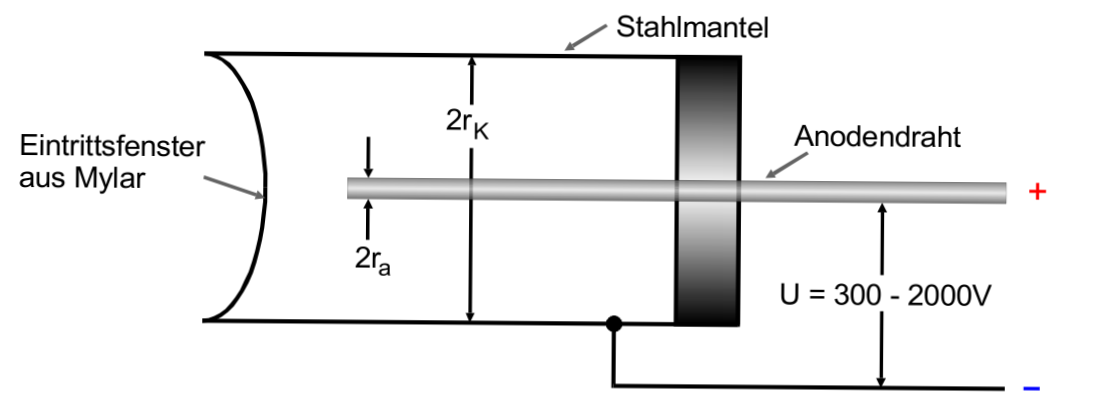
\includegraphics[scale=0.45]{zählrohr.png}
  \caption{Aufbau des Geiger-Müller-Zählrohrs.\cite{anleitung}}
  \label{fig:Geiger}
\end{figure}
\newline
Dringt ein Teilchen in das Zählrohrvolumen ein, sind die nach der Primärionisation ablaufenden
Vorgänge stark abhängig von der außen angelegten Spannung.
Wird eine geringe Spannung angelegt, geht ein großer Teil der Elektronen durch Rekombination
verloren. Bei größeren Spannungen hingegen nimmt die Rekombinationswahrscheinlichkeit ab, weshalb nahe
zu alle Elektronen den Anodendraht erreichen. Ionisationskammern werden bei diesen Spannungbereichen verwendet.
In diesem Bereich (Abb.2, Bereich II)ist der fließende Ionisationsstrom proportional zur Strahlungenergie und Strahlungsintensität.
\newline
Durch weitere Erhöhung der Spannung kommt es zum Vorgang der Stoßionisation. Hierbei können die freigesetzten
Elektronen genügend Energie aufnehmen, um ihrerseits ionisieren zu können. Bei hinreichend hoher Spannung kommt
es zum Vorgang der Townsed-Lawine, bei dem die Anzahl der freigesetzen Elektronen stark zunimmt.
In diesem Fall ist die pro Teilchen gesammelte Ladung Q so groß, dass der Ladunsimpuls als Maß für
die Teilchenenergie angesehen werden kann. Wegen der Proportionalität zwischen Ladung und Teilchenenergie
wird ein Proportionalitätrohr als Detektor verwendet (Abb.2, Bereich III)
\newline
Der Auslösebereich ist der eigentliche Arbeitsbereich des Geiger-Müller-Zählrohrs (Abb.2, Bereich IV). In diesem Bereich ist
die angelegte Spannung so groß, dass die Ladung unabhängig von der Primärionisation ist. Die Entladungen
breiten sich aufgrund von der hohen Anzahl entstandener UV-Photonen im gesamten Zählrohrvolumen aus. Dadurch
ist die gesammelte Ladung nicht mehr von der Primärionisation abhängig, sondern vom Zählrohrvolumen und der
angelegten Spannung. Aufgrund der nicht mehr vorhandenden Energieabhängigkeit können in diesem Bereich nur
Intensitätsmessung und keine Energiemessungen durchgeführt werden.
\newline
Durch die vielen Nachentladungen kann es bei nur einem ionisierenden Teilchen schon zu Dauerentladung kommen.
Dies ist der Bereich der selbstständigen Gasentladung (Abb.2, Bereich V), bei dem die hohen
Stromdichten schnell zur Zerstörung des Zählrohres führen können.
\begin{figure}
  \centering
  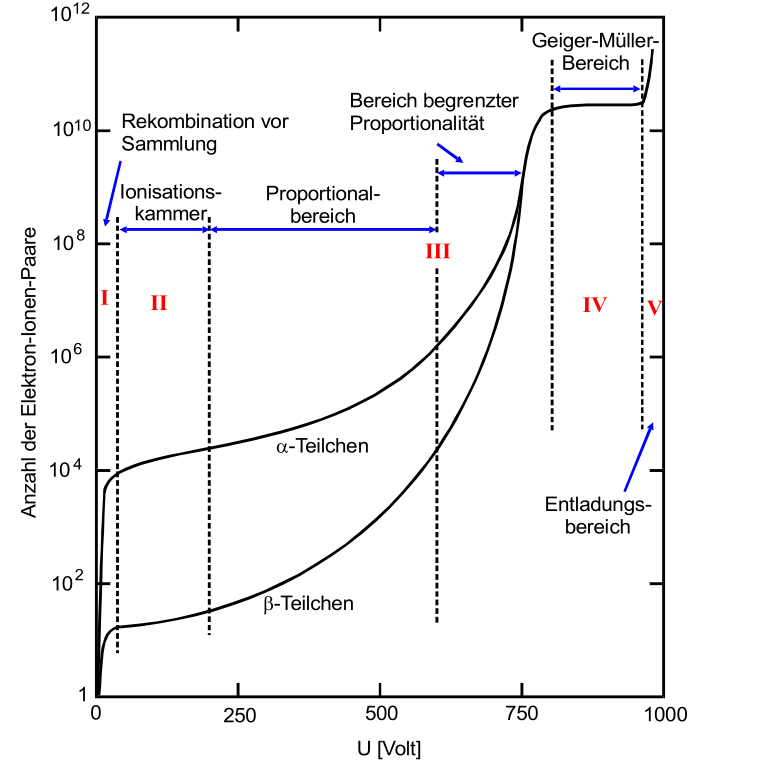
\includegraphics[scale=0.49]{bereiche.png}
  \caption{Bereiche abhängig von der Spannung.\cite{anleitung}}
  \label{fig:Bereiche}
\end{figure}
\newpage
\subsection{Einfluss der positiven Ionen}
In Abbildung \ref{fig:Zeit} ist der Einfluss der positiven Ionen innerhalb des Zählrohrs zu sehen.
Die positiven Ionen bauen vorrübergehend eine positive Radialladung zwischen Kathode und Anode auf.
Dies führt dazu, dass nahe des Drahts die Feldstärke für einige Zeit verringert wird, weshalb es zu keiner
Stoßionisation kommen kann. In der so genannten Totzeit T des Zählrohrs können eintreffende Teilchen
nicht registriert werden. An die Totzeit schließt sich die Erholungszeit $\su{T_E}$ an, bei der sich die positive
Ladung verringert und eine Lawinenbildung stufenweise möglich wird. Während dieser Zeit haben die Ausgangsimpulse
eine geringere Höhe. Erst im Anschluss an die Totzeit können die Ladungsimpule wieder ihre ursprüngliche
Höhe erreichen.
\newline
Ein weiterer Einfluss der positiven Ionen sind Nachentladungen. Diese sind zusätzlich auftretende Impulse,
die durch die Freisetzung von „Sekundärelektronen" entstehen. Sekundärelektronen entstehen, wenn Ionen aus
der Metalloberfläche Elektronen freisetzen. Diese Nachentladungen täuschen allerdings den Durchgang von
ionisierenden Teilchen vor. Durch die erwähnte Zugabe von Alkoholdämpfen im Zählrohr kann dieser Effekt
verringert werden. Die Ionen stoßen dann hauptsächlich mit Alkoholmolekülen. Die freiwerdende Energie
führt dann zur Schwingungsanregung der Alkoholmoleküle. Somit wird unter Zugabe der Alkohldämpfen
die freiwerdende Energie nicht für die Emission eines Elektrons verwendet, sondern in Bewegungsenergie
umgewandelt.
\begin{figure}
  \centering
  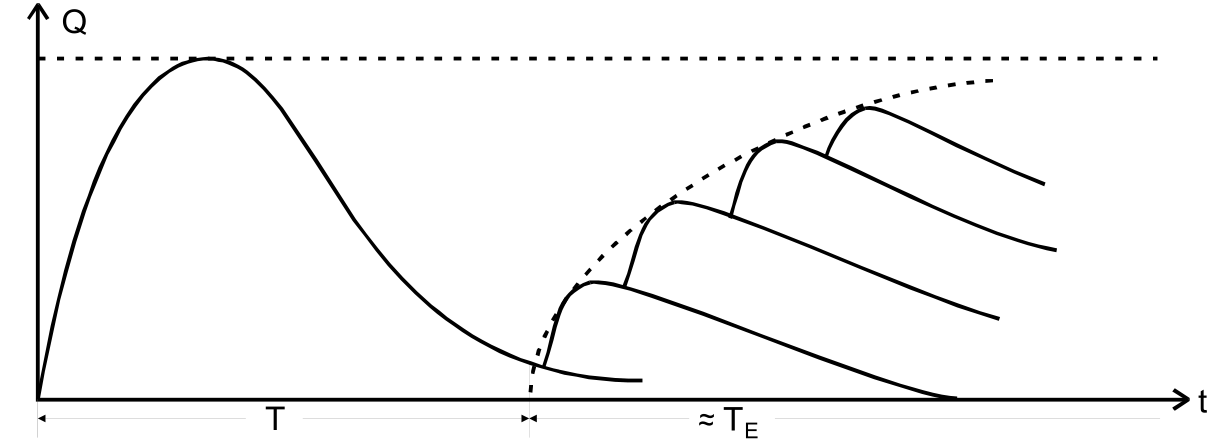
\includegraphics[scale=0.45]{erholungszeit.png}
  \caption{Tot-und Erholungszeit innerhalb eines Zählrohres.\cite{aneleitung}}
  \label{fig:Zeit}
\end{figure}

\subsection{Charakteristik des Zählrohrs}
Für die Charakteristik eines Geiger-Müller-Zählrohrs wird die registrierte Teilchenzahl N gegen die
angelegte Spannung U aufgetragen. Dies ist in Abbildung \ref{fig:Charakteristik} zu sehen.
\begin{figure}
  \centering
  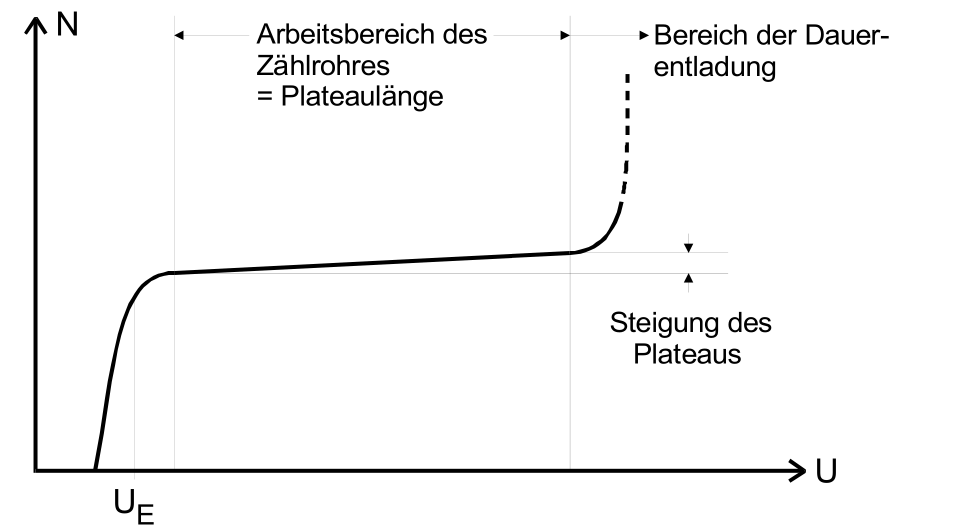
\includegraphics[scale=0.45]{charakteristik.png}
  \caption{Zählrohrcharakteristik bei konstanter Strahlungintensität.\cite{anleitung}}
  \label{fig:Charakteristik}
\end{figure}
Der Auslösebereich beginnt ungefähr bei der Spannug $\su{U_E}$, der dann durch den linearen Teil
der Kurve, das so genannte Plateau, forgesetzt wird. Anhand der Steigung und der Länge des Plateaus
kann eine Aussage über die Qualität des Zählrohrs getroffen werden. Im optimalen Fall wäre die Plateausteiguung
null. Trotz der Zugabe von Alkoholdämpfen ist dies durch Nachentladungen nicht möglich.
Mit immer größer werdender Spannung nimmt auch die Anzahl der Nachentladungen sehr stark zu.
An diesem Punkt geht es in den Bereich der Dauerentladung über.

\subsection{Ansprechvermögen des Zählrohres}
Das Ansprechvermögen ist die Wahrscheinlichkeit, dass ein einfallendes Teilchen im Zählrohr nachgewiesen
wird. Bei geladenen Teilchen, wie $\alpha$- und $\beta$-Teilchen ist das Ansprechvermögen bei nahezu 100 \%. Jedoch
werden sie durch ihre hohen Wechselwirkungen mit der Materie im Zählrohrmantel vollständig absorbiert.
Deshalb kommen Endfensterröhren zum Einsatz an deren Stirnseite Mylar-Folie angebracht ist, welche aus
Atomen mit niedriger Ordnungszahl besteht. Hier können selbst $\alpha$-Teilchen die Folie durchdringen und werden
nicht absorbiert.
\newpage
\section{Durchführung}
\begin{figure}
  \centering
  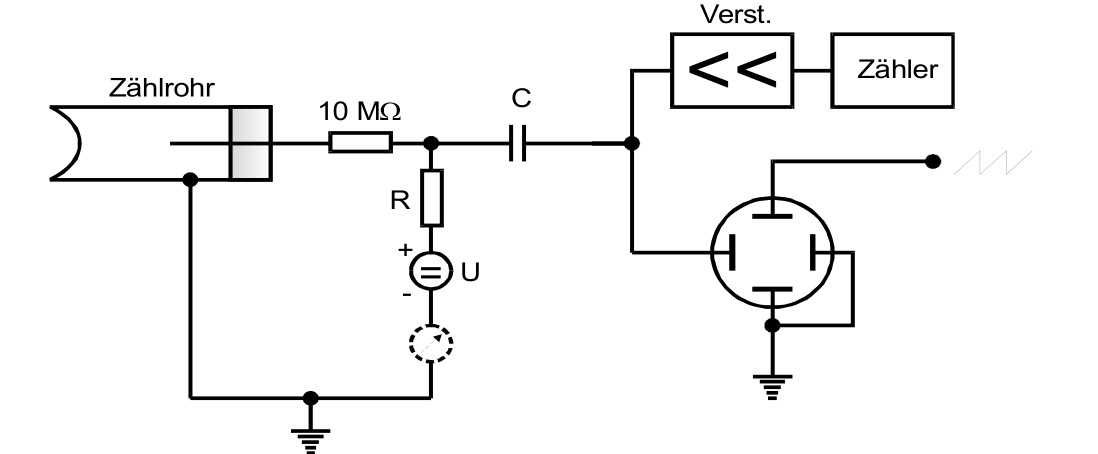
\includegraphics[scale=0.45]{aufbau.png}
  \caption{Versuchsaufbau.\cite{anleitung}}
  \label{fig:Aufbau}
\end{figure}
Der Versuch wird wie in Abbildung \ref{fig:Aufbau} aufgebaut. Dabei fließt die auf dem Zähldraht gesammelte Ladung Q
über den Widerstand R ab. Es entsteht ein Spannungsimpuls, der über einen Kondensator C ausgekoppelt,
im Verstärker vergrößert, im Zählgerät registriert und auf dem Oszillographen sichtbar gemacht wird.
\newline
Zuerst soll die Zählrate in Abhängigkeit von der Betriebsspannung bestimmt werden. Dafür
wird $\beta$-Quelle vor das Fenster der Zählrohres gestellt. Wichtig zu beachten ist, dass
die maximale Impulsrate nicht über 100/s steigt. Die Ionisierungsstrom und die Zählrate wird
in Abhängigkeit von der Spannung notiert.
\newline
Nun wird mithilfe des Oszillographen die Totzeit abgelesen und daraus die Erholunsgzeit bestimmt.
\newline
Als letztes wird mit der Zwei-Quellen-Methode die Totzeit bestimmt. Dafür wird die Zählrate $\symup{N_1}$
zuerst alleine gemessen, danach zusammen mit der Zählrate $\symup{N_2}$ und zum Schluss die
Zählrate $\symup{N_2}$ alleine.
